\newpage
\section{Ring buffer}

Ring buffer (hay gọi tiếng Việt là bộ đệm vòng) là một kĩ thuật được áp dụng rộng rãi trong lập trình nhúng.

Ví dụ bạn làm dự án mà MCU chính phải thực hiện giao tiếp với 4 đường UART, 1 đường I2C với 3 thiết bị ghép nối I2C, phải quét bàn phím, hiển thị lên LCD, giao tiếp với server qua giao thức MQTT\dots. Khi MCU đang quét bàn phím thì có dữ liệu trên cả 4 đường UART đến, MCU tạm dừng quét phím để xử lí dữ liệu vừa truyền tới. Sau đó MCU tiếp tục trở lại quét phím và không quét được 1 lần bạn ấn phím trước đó.

Trong những dự án lớn và đỏi hỏi nhiều tác vụ song song, việc xử lí không tốt các giao tiếp với ngoại vi làm mất mát dữ liệu đường truyền và hệ thống hoạt động không ổn định. Có rất nhiều kĩ thuật phải áp dụng để khiến hệ thống chạy trơn tru và đúng chức năng, Ring buffer là một trong các kĩ thuật đó.

Về ý tưởng thì Ring buffer là một bộ đệm dữ liệu, khi dữ liệu đến bất chợt mà không báo trước, bạn chỉ cần cất tất dữ liệu này vào bộ đệm. Sau khi thực hiện xong tác vụ quan trọng bạn có thể quay lại xử lí dữ liệu vừa nhận được trong bộ đệm.

\begin{wrapfigure}{l}{0.5\textwidth}
	\centering
    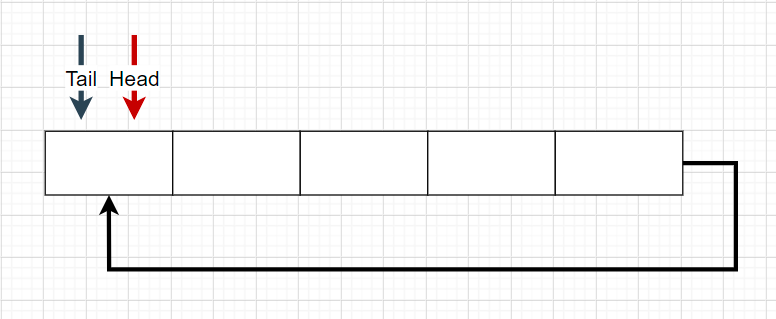
\includegraphics[width=0.5\textwidth]{Ringbuf.PNG}
\caption{Ringbuf empty}
\label{EmptyRingbuf}
\end{wrapfigure}

Ring buffer có cấu tạo gồm một mảng các ô nhớ như trên hình \ref{EmptyRingbuf} và hai con trỏ Head và Tail. Số lượng ô nhớ tùy thuộc vào khi bạn khởi tạo nó. Có hai tác vụ chính là Put (cất một byte vào bộ đệm) và Get (lấy 1 byte ra khỏi bộ đệm).

Khi khởi tạo con trỏ Head và Tail sẽ trỏ cùng vị trí vào ô nhớ đầu tiên của mảng.

Khi Put 1 byte vào bộ đệm, con trỏ Head dịch sang phải, đánh dấu vị trí sẽ lưu vào lần Put tiếp theo. Nếu Put 2 lần liên tiếp thì kết quả như trên hình \ref{RingbufPut}.

\begin{figure}[h!]
    \centering
    \subfloat[Ringbuf Put]{
        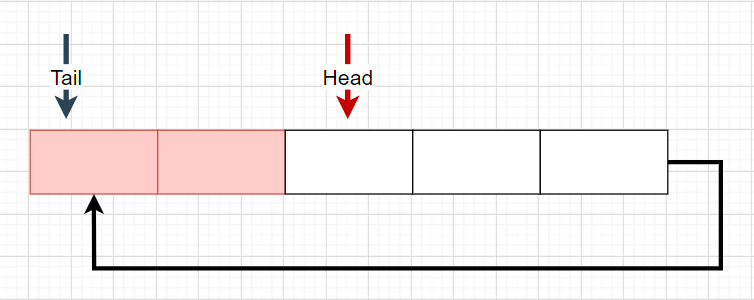
\includegraphics[width=0.5\textwidth]{RingbufPut2.PNG}
        \label{RingbufPut}
    }
    \subfloat[Ringbuf Get]{
        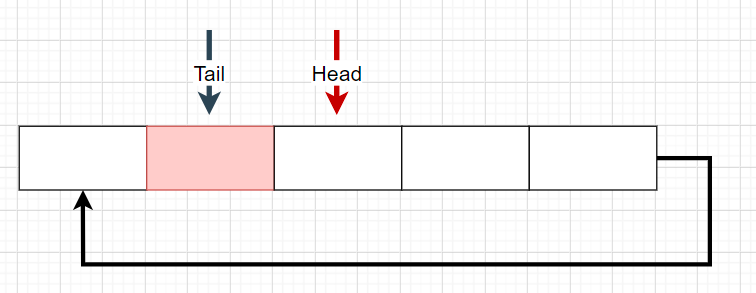
\includegraphics[width=0.5\textwidth]{RingbufGet1.PNG}
        \label{RingbufGet}
    }
    \caption{Ringbuf}
\end{figure}

Khi Get 1 byte, nếu bộ đệm có dữ liệu, bộ đệm sẽ trả về byte tại vị trí của con trỏ Tail, đồng thời dịch chuyển con trỏ này sang phải, đánh dấu vị trí của lần Get sau. Hình \ref{RingbufGet}. Như vậy dữ liệu đã đi đúng theo thư tự byte đến trước sẽ được Get ra trước.

Khi con trỏ Head vượt quá phần tử cuối cùng của mảng thì nó quay trở lại phần tử đầu tiên và tiếp tục công việc của mình. Hình \ref{HeadReturn}

Với cách hoạt động trên, bộ đệm rỗng khi con trỏ Head và Tail trùng nhau hình \ref{EmptyRingbuf}, bộ đệm sẽ đầy khi con trỏ Head nằm ngay sau con trỏ Tail. Bạn có thể thấy dù còn 1 ô nhớ trống như hình \ref{RingbufFull}  Đến lúc này bạn sẽ không Put dữ liệu vào được nữa và gây mất mát dữ liệu.

Có nhiều cách khắc phục tình trạng trên. Bao gồm viết chương trình theo dạng Non-Blocking, cấp mảng lớn hơn cho bộ đệm, quy định dữ liệu tối đa mà MCU có thể nhận trong một khoảng thời gian\dots.

\begin{figure}[h!]
    \centering
    \subfloat[Head return]{
        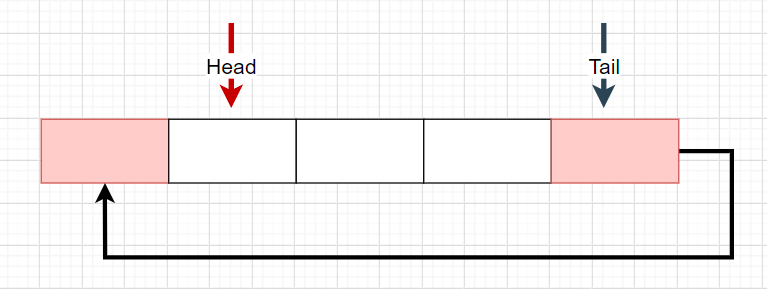
\includegraphics[width=0.5\textwidth]{RingbufBack.PNG}
        \label{HeadReturn}
    }
    \subfloat[Ringbuf full]{
        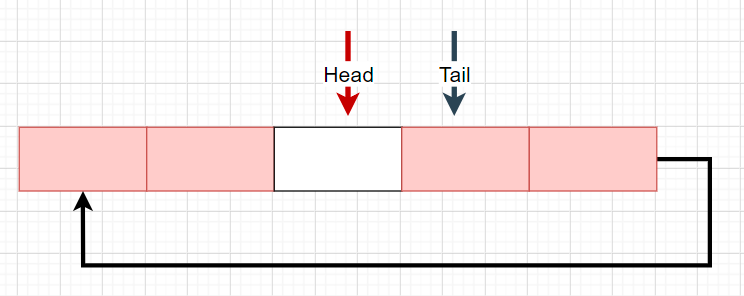
\includegraphics[width=0.5\textwidth]{RingbufFull.PNG}
        \label{RingbufFull}
    }
    \caption{Ringbuf}
\end{figure}

Thông thường, lệnh Put sẽ được thực hiện trong tác vụ ngắt của UART hoặc các giao thức truyền thông khác. Còn lệnh Get sẽ được thực hiện trong vòng lặp chính, lúc này MCU sẽ đọc hết dữ liệu ra và xử lí.

\begin{figure}[h!]
    \centering
    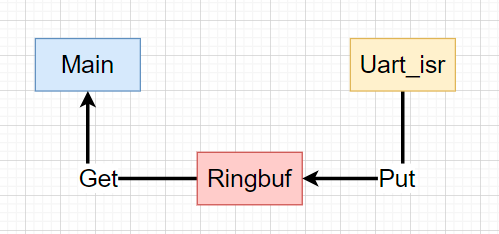
\includegraphics[width=0.5\textwidth]{RingbufFlow.PNG}
\end{figure}

